\documentclass[11pt,a4paper]{article}

% Impostazioni per la codifica e la lingua
\usepackage[utf8]{inputenc}   % Codifica UTF-8
\usepackage[T1]{fontenc}      % Font in T1
\usepackage[italian]{babel}   % Lingua italiana
\usepackage{lmodern}          % Font moderni
\usepackage{url}

% Pacchetti matematici e grafici
\usepackage{amsmath,amssymb}  % Simboli matematici
\usepackage{graphicx}         % Inclusione di immagini

% Impostazioni di layout
\usepackage{geometry}         
\geometry{a4paper, margin=2.5cm}

% Titolo, autore e data
\title{Assistente alimentare: generatore di lista della spesa}
\author{Gabriele Adorni}
\date{\today}

\begin{document}

% -----------------------
%  PRIMA PAGINA (FRONTESPIZIO)
% -----------------------
\begin{titlepage}
    \begin{center}
        \vspace*{1cm}
        % Inserisci il nome esatto del file immagine (senza estensione .png se preferisci)
        
\includegraphics[width=6cm]{polito_logo.png}\\[2cm]

        \textsc{\LARGE POLITECNICO DI TORINO}\\[0.8cm]
        \textsc{Dipartimento di Ingegneria Gestionale e della Produzione}\\[2cm]

        \textsc{Corso di Laurea Triennale in Ingegneria Gestionale}\\
        \textsc{Classe L-8 Ingegneria dell’Informazione}\\[2cm]

        {\Large\textsc{\textbf{Prova Finale}}\\[1cm]}
        
        {\Large \textbf{Assistente alimentare: \textit{tool} per la generazione\\
        di una lista della spesa ottimizzata}}\\[3cm]

        \begin{flushleft} \large
            \textbf{Relatore:}\\
            Professor Giuseppe Bruno Averta
        \end{flushleft}

        \begin{flushright} \large
            \textbf{Candidato:}\\
            Gabriele Adorni\\
            Matricola: s297466
        \end{flushright}

        \vfill

        \textsc{Marzo 2025}

    \end{center}
\end{titlepage}

% Indice (Table of Contents)
\tableofcontents
\newpage

% ====================================================
% CAPITOLO 1 (GIÀ FATTO)
% ====================================================
\section{Proposta di progetto}

\subsection{Titolo della proposta}
Assistente alimentare: generatore di lista della spesa

\subsection{Descrizione del problema proposto}
Il progetto affronta la problematica della creazione di un’applicazione in grado di generare una lista di prodotti alimentari il cui apporto complessivo di nutrienti e calorie soddisfi il fabbisogno giornaliero dell’individuo, tenendo conto anche delle preferenze personali. L’obiettivo dell’applicazione è sollevare l’utente dall'onere di dover ideare quotidianamente una lista della spesa bilanciata: l’\textit{App} provvederà a generarla, valutando lo stato fisico, gli obiettivi nutrizionali e le preferenze alimentari dell’utente.\\
Per fare ciò l’utente dovrà fornire alcune informazioni biometriche e rispondere a domande relative al proprio stile di vita; da questi dati verranno calcolati i parametri necessari per ottimizzare la lista della spesa, che potrà essere in seguito modificata a condizione che il bilanciamento nutrizionale complessivo venga mantenuto.

\subsection{Descrizione della rilevanza gestionale del problema}
In un’epoca in cui la correlazione tra nutrizione e salute è ormai consolidata, l’applicazione si propone come uno strumento utile per semplificare la gestione di una corretta alimentazione. Essa funge da assistente alimentare, consentendo all’utente di strutturare la propria lista della spesa in conseguenza della propria dieta, seguendo solide linee guida che rappresentano le fondamenta e i vincoli degli algoritmi impiegati per generare l’\textit{output} finale. Tale approccio non solo mira a garantire un risparmio di tempo nella routine quotidiana, ma contribuisce anche a migliorare lo stile di vita e la salute, nonché a consolidare consapevolezze in campo alimentare.

\subsection{Descrizione del \textit{dataset} per la valutazione}
La scelta del \textit{dataset} per la valutazione non è stata semplice. Durante la ricerca su siti web che offrono \textit{dataset} open-source (ad esempio, Kaggle) si è riscontrata una maggiore presenza di \textit{dataset} di stampo commerciale, contenenti prodotti alimentari provenienti da supermercati e aziende, corredati da informazioni non strettamente utili all’applicazione (come prezzi di vendita, percentuali di sconto, quantità vendute…). Tra le opzioni orientate all’aspetto nutrizionale, è stato selezionato il seguente (https://www.kaggle.com/datasets/utsavdey1410/food-nutrition-dataset).\\
Successivamente, è stato necessario effettuare alcune operazioni di \textit{data management} per conformare il \textit{dataset} alle specifiche richieste dall’applicazione. In particolare, le cinque tabelle (FOOD DATA GROUP.csv) contenute nel \textit{dataset} sono state unite, aggiungendo una colonna con una chiave univoca per identificare ciascun prodotto, e rimuovendo alcune colonne ritenute superflue. Inoltre, per aggiungere un ulteriore livello di personalizzazione per l’utente, è stata integrata una tabella aggiuntiva nel database contenente la chiave univoca del prodotto, il relativo nome e numerose colonne con valori booleani che indicano l’aderenza del prodotto a determinati requisiti, sia relativi a preferenze dietetiche (ad es. dieta vegana/non vegana) sia a condizioni mediche (ad es. presenza o assenza di lattosio). Durante le fasi di sviluppo e test dell’applicazione sono state inoltre eliminate alcune classi di prodotti non conformi alle fondamenta etiche del progetto, come quelli provenienti da \textit{fast-food} o relativi ad alcolici.

\subsection{Descrizione preliminare degli algoritmi coinvolti}

\textbf{Calcolo del fabbisogno calorico e nutrizionale}\\
L’algoritmo prenderà in \textit{input} i dati personali dell’utente, quali peso, altezza, età, sesso e livello di attività fisica. Sulla base di queste informazioni verrà utilizzata una formula standard, ad esempio l’equazione di Harris-Benedict o quella di Mifflin-St Jeor, per calcolare il TDEE (\textit{Total Daily Energy Expenditure}), ovvero il fabbisogno calorico giornaliero. Successivamente il fabbisogno calorico verrà suddiviso tra i macronutrienti (proteine, carboidrati e grassi) secondo proporzioni personalizzabili o basate su raccomandazioni standard (ad es. 30\% proteine, 50\% carboidrati, 20\% grassi). In corso d’opera è stato aggiunto il calcolo dell’apporto di fibre e di alcuni micronutrienti.

\bigskip
\textbf{Ottimizzazione lineare}\\
Utilizzando il TDEE e i fabbisogni giornalieri di nutrienti precedentemente calcolati, l’algoritmo genererà una lista della spesa che soddisfi le esigenze nutrizionali dell’utente. Tale processo verrà strutturato come un problema di programmazione lineare, con una funzione obiettivo che minimizza la differenza tra il fabbisogno nutrizionale e il contributo degli alimenti. Durante la fase di sviluppo sono state esplorate diverse soluzioni per la ricerca di combinazioni di prodotti ottimali o subottimali, inclusa una strategia basata su una funzione ricorsiva \textit{greedy}, arricchita da euristiche per semplificare e velocizzare il calcolo. Tuttavia l’approccio basato sulla programmazione lineare si è rivelato il più efficace, consentendo quest'ultimo di ottenere soluzioni subottimali molto vicine all’ottimo in tempi ragionevoli.

\subsection{Descrizione preliminare delle funzionalità previste per l’applicazione \textit{software}}

L’applicazione sarà progettata con un’interfaccia utente semplice e intuitiva, offrendo le seguenti funzionalità:
\begin{enumerate}
    \item \textbf{Inserimento delle informazioni personali}\\
    L’utente potrà fornire dettagli quali peso, altezza, sesso, età e livello di attività fisica. Una volta inseriti correttamente, questi dati permetteranno di calcolare il TDEE (fabbisogno calorico giornaliero), che costituirà la base per la strutturazione di un piano alimentare. Per chi desidera una maggiore personalizzazione, sarà possibile aumentare o diminuire il valore calorico giornaliero in incrementi di 100 calorie, così da generare una lista coerente con una dieta iper o ipocalorica.
    
    \item \textbf{Preferenze alimentari}\\
    Prima della generazione della lista, l’utente potrà personalizzare l’\textit{output} attivando degli ``switch'' per includere o escludere determinate categorie di prodotti nell’ottimizzazione. Tali categorie saranno legate sia a preferenze dietetiche (ad es. dieta vegana) sia a condizioni mediche (ad es. presenza o assenza di lattosio nei prodotti).
    
    \item \textbf{Generazione della lista}\\
    Attraverso un apposito pulsante, l’utente potrà avviare la generazione della lista della spesa, la quale verrà visualizzata a schermo accompagnata da un istogramma che evidenzia le prestazioni dell’ottimizzazione. Per ciascun nutriente verrà mostrata una colonna che rappresenta il \textit{target} e una colonna che indica il totale fornito dagli alimenti, con l’obiettivo di mantenere l’equilibrio.
    
    \item \textbf{Ulteriore personalizzazione dell’output}\\
    Dopo la generazione dell’\textit{output}, l’utente potrà personalizzare ulteriormente la propria esperienza accedendo a una sezione dedicata. In questa sezione sarà possibile effettuare un ``refresh'' completo dell’\textit{output} oppure sostituire alcuni prodotti indesiderati con altri aventi un profilo nutrizionale simile, in modo da non compromettere il bilanciamento complessivo.
    
    \item \textbf{Sezione informativa/carenze nutrizionali}\\
    L’ultima sezione dello strumento consentirà all’utente di colmare eventuali carenze di alcuni micronutrienti. Selezionando un nutriente (tra quelli non ottimizzati per evitare un’eccessiva complessità computazionale), l’utente potrà accedere a una descrizione degli effetti di quel nutriente e alle motivazioni per cui è importante assumerlo in una determinata quantità, oltre a ricevere una lista di prodotti che lo contengono, ordinata in ordine decrescente in base alla quantità presente.
\end{enumerate}

% ====================================================
% CAPITOLO 2
% ====================================================
\section{Descrizione dettagliata del problema affrontato}

\subsection{Contesto di utilizzo dell’applicazione}
Per l'individuo adulto medio, l'attività del "fare la spesa" rappresenta un compito quotidiano imprescindibile, che richiede una pianificazione accurata e l'impiego di tempo ed energie. Spesso, tuttavia, tale impegno non porta a risultati ottimali, a causa di una carenza di competenze specifiche o di altre difficoltà organizzative.\\[0.5em]
L'applicazione si propone di generare automaticamente una lista della spesa ottimizzata, in grado di assicurare un apporto nutrizionale bilanciato e perfettamente in linea con le esigenze individuali. In particolare, il sistema raccoglie dati biometrici e informazioni sulle preferenze alimentari dell'utente per elaborare un output completamente personalizzato. Se progettato e implementato correttamente, uno strumento di questo tipo potrà apportare notevoli benefici, non solo in termini di comodità, ma soprattutto per il miglioramento della salute di chi lo utilizza.

\subsection{Come si produce una dieta bilanciata}
La creazione di una dieta equilibrata parte dalla corretta valutazione del fabbisogno energetico individuale, definito attraverso il calcolo del metabolismo basale (BMR) e del fabbisogno calorico totale giornaliero (TDEE). È fondamentale semplificare il concetto di ``alimentazione'', considerando che ogni alimento è caratterizzato da due aspetti essenziali: un apporto energetico (solitamente espresso in kilocalorie) e un apporto nutrizionale, ossia la composizione in nutrienti quali proteine, carboidrati, grassi e micronutrienti (vitamine e minerali). Questi elementi, analizzati in base alle etichette nutrizionali (tipicamente per 100 g di prodotto), costituiscono la base per determinare la combinazione ottimale di alimenti che soddisfi il fabbisogno individuale.

\subsubsection{Composizione degli alimenti}
I prodotti alimentari si caratterizzano per la presenza di nutrienti essenziali, suddivisi in due categorie principali: macronutrienti e micronutrienti. I macronutrienti comprendono carboidrati, proteine e grassi, che forniscono l'energia necessaria per il funzionamento quotidiano dell'organismo. I micronutrienti, invece, includono vitamine e minerali, fondamentali per il corretto svolgimento delle funzioni fisiologiche, pur essendo necessari in quantità minori.\\[0.5em]
Le informazioni nutrizionali riportate sulle etichette degli alimenti, solitamente espresse per 100 g di prodotto, forniscono una panoramica dettagliata del contenuto di ciascun nutriente. Tali tabelle permettono di parametrare in maniera oggettiva il contributo di ogni alimento al fabbisogno giornaliero consigliato.\\[0.5em]
Il sistema utilizza questi dati nutrizionali per selezionare una combinazione di alimenti che, complessivamente, raggiunga i livelli raccomandati di nutrienti. In altre parole, l'obiettivo è quello di combinare prodotti con differenti profili nutrizionali in modo che il totale assorbito soddisfi sia i requisiti energetici (forniti dai macronutrienti) sia il fabbisogno di micronutrienti indispensabili per la salute. Questo approccio permette di pianificare diete equilibrate, che contribuiscono al benessere generale e alla prevenzione di carenze nutrizionali.

\subsubsection{TDEE e BMR}
Il metabolismo basale (BMR) rappresenta l’energia minima necessaria per mantenere in funzione le attività vitali a riposo (ad esempio, respirazione, circolazione sanguigna e mantenimento della temperatura corporea). Per calcolare il BMR si utilizzano formule che richiedono input quali peso, altezza, età e sesso. Tra le formule più note troviamo: 
\begin{itemize}
  \item \textbf{Formula di Harris-Benedict (versione originale):}
    \begin{itemize}
      \item Per gli uomini: 
        \[
        \text{BMR} = 66 + (13,7 \times \text{peso [kg]}) + (5 \times \text{altezza [cm]}) - (6,8 \times \text{età [anni]})
        \]
      \item Per le donne: 
        \[
        \text{BMR} = 655 + (9,6 \times \text{peso [kg]}) + (1,8 \times      \text{altezza [cm]}) - (4,7 \times \text{età [anni]})
        \]
    \end{itemize}
  \item \textbf{Formula di Mifflin-St Jeor (considerata più accurata):}
    \begin{itemize}
      \item Per gli uomini: 
        \[
        \text{BMR} = (10 \times \text{peso [kg]}) + (6,25 \times \text{altezza [cm]}) - (5 \times \text{età [anni]}) + 5
        \]
      \item Per le donne: 
        \[
        \text{BMR} = (10 \times \text{peso [kg]}) + (6,25 \times \text{altezza [cm]}) - (5 \times \text{età [anni]}) - 161
        \]
    \end{itemize}
\end{itemize}
Il \textit{Total Daily Energy Expenditure} (TDEE) rappresenta il fabbisogno calorico totale giornaliero, includendo sia l'energia necessaria per le funzioni vitali (BMR) sia quella spesa nelle attività quotidiane. Per calcolare il TDEE, il BMR viene moltiplicato per un coefficiente di attività fisica (AF) che varia in base al livello di attività dell'individuo. I valori tipici del coefficiente di attività sono:
\begin{itemize}
  \item Sedentario: AF $\approx$ 1.2
  \item Leggermente attivo: AF $\approx$ 1.375
  \item Moderatamente attivo: AF $\approx$ 1.55
  \item Molto attivo: AF $\approx$ 1.725
  \item Estremamente attivo: AF $\approx$ 1.9
\end{itemize}
La formula finale è quindi:
\[
\text{TDEE} = \text{BMR} \times \text{AF}
\]
Il TDEE non solo rappresenta il quantitativo di energia necessario per mantenere il peso corporeo stabile, ma funge anche da parametro di riferimento per raggiungere specifici obiettivi di variazione del peso. Infatti se l'apporto calorico giornaliero supera il TDEE, l'eccesso energetico viene immagazzinato (generalmente sotto forma di grasso), portando ad un aumento di peso. Al contrario, un apporto inferiore al TDEE genera un deficit calorico che, se prolungato, si traduce in una perdita di peso. Questi calcoli, basati sui dati biometrici e sul livello di attività fisica dell’utente, forniscono il valore energetico totale su cui si fonda la pianificazione nutrizionale.

\subsubsection{Calcolo dei fabbisogni nutrizionali per i singoli nutrienti}
Per ottenere una dieta bilanciata è essenziale definire con precisione il quantitativo di ciascun nutriente da assumere giornalmente. L'approccio adottato si basa sulla suddivisione del fabbisogno energetico totale (TDEE) e su parametri individuali (peso, sesso, età) per determinare i requisiti di macronutrienti e micronutrienti, seguendo linee guida nutrizionali scientificamente validate.
\begin{itemize}
  \item \textbf{Macronutrienti:}
    \begin{itemize}
      \item \textbf{Grassi:} si prevede che circa il 30\% delle calorie totali debba provenire dai grassi. Poiché ogni grammo di grassi fornisce circa 9 kcal, il quantitativo in grammi si ottiene moltiplicando il TDEE per 0.3 e dividendolo per 9.
      \item \textbf{Grassi Saturi:} viene assegnato il 10\% del TDEE a questo sotto-gruppo, anch’esso convertito in grammi dividendo per 9.
      \item \textbf{Carboidrati:} con il 50\% del TDEE destinato ai carboidrati e considerando che ogni grammo fornisce 4 kcal, il fabbisogno in grammi si calcola moltiplicando il TDEE per 0.5 e dividendolo per 4.
      \item \textbf{Proteine:} il fabbisogno proteico viene determinato in base al peso corporeo, con coefficienti differenziati in base al sesso (0.8 g/kg per le donne e 1.0 g/kg per gli uomini) per riflettere le diverse esigenze metaboliche.
    \end{itemize}
  \item \textbf{Micronutrienti e altri componenti:}
    \begin{itemize}
      \item \textbf{Fibra:} vengono assegnati valori fissi (25 g per le donne e 30 g per gli uomini) che supportano la regolarità intestinale e il benessere generale.
      \item \textbf{Sodio:} il quantitativo raccomandato varia in funzione dell'età (1500 mg per individui sotto i 50 anni e 1300 mg per quelli oltre), in linea con le raccomandazioni per il controllo della pressione arteriosa.
      \item \textbf{Vitamina C:} la dose giornaliera è fissata a 75 mg per le donne e 90 mg per gli uomini, in base alle necessità antiossidanti e al supporto del sistema immunitario.
      \item \textbf{Vitamina D:} viene stabilito un fabbisogno di 15 microgrammi, fondamentale per il metabolismo del calcio e la salute delle ossa.
      \item \textbf{Calcio:} un apporto standard di 1000 mg al giorno è considerato adeguato per il mantenimento della densità ossea.
      \item \textbf{Ferro:} le esigenze di ferro sono maggiori nelle donne (18 mg) rispetto agli uomini (8 mg), in considerazione delle perdite ematiche e delle necessità ematologiche.
      \item \textbf{Potassio:} i valori raccomandati sono 3400 mg per gli uomini e 2600 mg per le donne, essenziali per il corretto funzionamento muscolare e la regolazione della pressione arteriosa.
    \end{itemize}
\end{itemize}
L'approccio matematico, basato su proporzioni di energia e pesi specifici, permette di tradurre in valori quantitativi raccomandati le linee guida nutrizionali internazionali, garantendo un \textit{output} personalizzato e scientificamente fondato. La suddivisione scelta consente di rispettare sia il fabbisogno energetico (espresso in kcal) sia quello nutrizionale (composto dai singoli nutrienti), offrendo così una base solida per la generazione di una lista della spesa che soddisfi in modo ottimale le esigenze dell’utente.

\subsection{Funzionamento pratico dell’assistente alimentare}
L’assistente alimentare è strutturato in quattro sezioni operative che guidano l’utente dalla definizione dei propri dati biometrici fino alla personalizzazione finale della lista della spesa, garantendo un processo intuitivo e flessibile.
\begin{itemize}
  \item \textbf{Prima sezione.} L’utente inserisce i propri dati biometrici, fondamentali per il calcolo del TDEE. Una volta validati, il sistema calcola il fabbisogno calorico in kilocalorie. L’utente può poi regolare questo valore, incrementandolo o decrementandolo di 100 kcal per volta, fino a raggiungere un apporto calorico giornaliero coerente con i propri obiettivi. È altresì possibile filtrare gli elementi del \textit{database} per escludere prodotti indesiderati o non conformi alla propria dieta, sia per scelte personali (ad es., dieta vegana) sia per particolari esigenze (ad es. intolleranze al lattosio).
  \item \textbf{Seconda sezione.} In questa fase l’utente avvia la ricerca di una combinazione di alimenti che soddisfi il proprio fabbisogno calorico. Il sistema genera un \textit{output} visualizzato come una lista in cui per ciascun alimento sono indicati il nome e le porzioni suggerite. Se l’\textit{output} non risponde alle aspettative, è possibile effettuare un ``refresh'' per rigenerare una nuova proposta. Contestualmente viene presentato un grafico (istogramma) che confronta il \textit{target} nutrizionale con il totale dei nutrienti forniti dalla lista, offrendo così una valutazione immediata dell’efficacia dell’ottimizzazione.
  \item \textbf{Terza sezione.} L’utente accede a una finestra contenente l’\textit{output} generato, con la possibilità di personalizzare la lista. In questa fase è possibile sostituire uno o più prodotti, purché il nuovo alimento proposto sia nutrizionalmente simile a quello rimosso, per mantenere l’equilibrio della dieta. Una volta apportate le modifiche desiderate, l’utente le conferma, aggiornando l’\textit{output} sia nella lista che nel grafico, che verranno riproposti nella sezione precedente.
  \item \textbf{Quarta sezione.} Questa parte, concepita principalmente a scopo informativo, fornisce gli strumenti per colmare eventuali carenze nutrizionali già note all’utente. Selezionando un micronutriente dalla lista disponibile, il sistema mostra la lista degli alimenti presenti nel \textit{database} che lo contengono, specificandone anche la quantità, accompagnata da una breve spiegazione della funzione principale del nutriente. Questo consente all’utente di approfondire il proprio profilo nutrizionale e di integrare la dieta in modo mirato.
\end{itemize}

\subsection{Criticità}  
Tra le principali criticità si evidenzia l’importanza di disporre di un \textit{dataset} di alta qualità. La correttezza e l’accuratezza dei dati nutrizionali e dei parametri biometrici sono fondamentali per garantire un \textit{output} valido e affidabile. Errori o imprecisioni nei dati possono compromettere il calcolo del TDEE e la suddivisione dei fabbisogni nutrizionali, influendo negativamente sull’ottimizzazione finale. Un’altra criticità riguarda la complessità nell’integrare preferenze, restrizioni e variabili individuali in un modello matematico robusto e allo stesso tempo flessibile.

\subsection{Potenzialità e rilevanza}  
Il \textit{tool} presenta numerose potenzialità, sia per l’utente singolo sia per le aziende:
\begin{itemize}
  \item \textbf{Salute e benessere:} offrendo un supporto per la pianificazione di diete equilibrate, lo strumento contribuisce al miglioramento della salute degli utenti e alla prevenzione di carenze nutrizionali.
  \item \textbf{Informazione e cultura alimentare:} la possibilità di visualizzare e comprendere il bilanciamento nutrizionale dei pasti favorisce una maggiore consapevolezza e informazione in tema di alimentazione sana.
  \item \textbf{Innovazione e competitività:} per le piattaforme di spesa online, l’integrazione di un sistema di generazione automatica della lista della spesa può rappresentare un vantaggio competitivo, migliorando l’esperienza utente e differenziando l’offerta nel mercato.
\end{itemize}
In sintesi, il \textit{tool} intende configurarsi come uno strumento versatile e innovativo, capace di rispondere a esigenze diverse e di avere un impatto positivo sia a livello individuale che aziendale, favorendo una gestione più consapevole e personalizzata dell’alimentazione.


% (Sottocapitoli da definire in seguito)

% ====================================================
% CAPITOLO 3
% ====================================================
\section{Descrizione del \textit{dataset} utilizzato per l’analisi}
Il \textit{dataset} rappresenta un elemento fondamentale per il funzionamento dell’applicazione, in quanto fornisce, attraverso \textit{query} mirate, informazioni dettagliate sui prodotti alimentari. Queste informazioni vengono successivamente convertite in oggetti della classe \textit{Food}, costituendo la base per la generazione automatica di una lista della spesa ottimizzata. In questo contesto, il \textit{dataset} non solo costituisce la fonte primaria dei dati nutrizionali, ma svolge anche un ruolo determinante nel garantire la qualità e la coerenza dei risultati ottenuti dall’applicazione.

\subsection{Ricerca del \textit{dataset}}
Il processo di ricerca del \textit{dataset} ha avuto inizio con l’esplorazione di diverse piattaforme \textit{online}, tra cui Kaggle e altre risorse similari, dove erano disponibili numerosi \textit{dataset} relativi ai prodotti alimentari. Molti di questi presentavano una struttura monolitica, composta da una singola tabella contenente informazioni quali: nome del cibo, peso, calorie, proteine, ecc.. Tuttavia, i requisiti specifici del progetto imponevano la presenza di ulteriori elementi, quali un valore di porzione tipica e categorie esplicative (ad es. etichette per identificare latticini, prodotti vegani, ecc.), oltre ai dettagli sui nutrienti e micronutrienti.

Nessuno dei \textit{dataset} disponibili rispondeva pienamente a tali requisiti; pertanto, è stato scelto un \textit{dataset} che, pur non essendo perfetto, soddisfaceva i requisiti fondamentali. Successivamente è stato sottoposto a processi di \textit{data management} e \textit{data cleaning} per adattarlo alle specifiche esigenze dell’applicazione. Le modifiche apportate saranno illustrate in dettaglio nelle sezioni successive.

\subsection{Descrizione del \textit{dataset} scelto}
Il \textit{dataset} originario è disponibile al seguente link:
\begin{center}
\url{https://www.kaggle.com/datasets/utsavdey1410/food-nutrition-dataset}
\end{center}
Il materiale, in lingua inglese, comprende cinque file \texttt{.csv} contenenti informazioni nutrizionali relative a diversi alimenti.

\subsubsection{Modifiche effettuate al \textit{dataset}}
I file \texttt{.csv} sono stati uniti e rielaborati tramite la libreria \textit{pandas}, con l’obiettivo di:
\begin{itemize}
    \item Creare un’unica tabella che riunisse i dati provenienti dalle cinque sorgenti.
    \item Assegnare una chiave primaria (\texttt{ID}) a ciascun alimento, utile per l’identificazione univoca all’interno del database.
    \item Rimuovere le colonne superflue, non rilevanti per l’ottimizzazione o la generazione della lista della spesa.
\end{itemize}

Dopo questi interventi di \textit{data cleaning} e \textit{data management}, la tabella risultante (denominata, ad esempio, \texttt{food\_nutrients}) si presenta con i seguenti attributi principali:
\begin{itemize}
    \item \textbf{ID}: identificatore numerico univoco (\textit{primary key}).
    \item \textbf{Food}: nome dell’alimento.
    \item \textbf{Caloric Value}: energia totale fornita dall’alimento, in kcal per 100 g.
    \item \textbf{Fat (in g)}: quantità totale di grassi in grammi per 100 g, comprensiva di sottocategorie.
    \item \textbf{Saturated Fats (in g)}: quantità di grassi saturi per 100 g.
    \item \textbf{Monounsaturated Fats (in g)}: quantità di grassi monoinsaturi per 100 g.
    \item \textbf{Polyunsaturated Fats (in g)}: quantità di grassi polinsaturi per 100 g.
    \item \textbf{Carbohydrates (in g)}: totale dei carboidrati in grammi per 100 g.
    \item \textbf{Sugars (in g)}: zuccheri semplici in grammi per 100 g.
    \item \textbf{Protein (in g)}: contenuto proteico per 100 g.
    \item \textbf{Dietary Fiber (in g)}: contenuto di fibre alimentari per 100 g.
    \item \textbf{Cholesterol (in mg)}: colesterolo per 100 g.
    \item \textbf{Sodium (in mg)}: sodio per 100 g.
    \item \textbf{Water (in g)}: acqua in grammi per 100 g.
    \item \textbf{Vitamin A, B1, B2, \ldots, B12, C, D, E, K (in mg)}: vitamine essenziali.
    \item \textbf{Calcium, Iron, Magnesium, \ldots, Zinc (in mg)}: minerali essenziali.
    \item \textbf{Nutrition Density}: indice di densità nutrizionale per caloria.
\end{itemize}

\subsubsection{Realizzazione della tabella preferenze}
Durante la fase di sviluppo del progetto, è emersa l’esigenza di implementare un sistema di filtraggio dei cibi in base alle preferenze dell’utente (ad es. alimenti vegani, vegetariani, senza lattosio, ecc.). Per questo motivo, è stata creata una tabella \texttt{food\_preferences}, definita manualmente, con la seguente struttura:
\begin{itemize}
    \item \textbf{ID}: identificatore univoco (\textit{primary key}).
    \item \textbf{Food}: nome dell’alimento.
    \item \textbf{Vegano}: valore 1 se l’alimento non contiene ingredienti di origine animale, 0 altrimenti.
    \item \textbf{Vegetariano}: valore 1 se l’alimento non contiene carne, pesce o pollame (ma può includere latte e uova), 0 altrimenti.
    \item \textbf{Lattosio}: valore 1 se l’alimento contiene derivati del latte, 0 altrimenti.
    \item \textbf{Glutine}: valore 1 se l’alimento contiene cereali contenenti glutine, 0 altrimenti.
    \item \textbf{Arachidi}: valore 1 se l’alimento contiene arachidi, 0 altrimenti.
    \item \textbf{Frutta secca}: valore 1 se l’alimento include noci, mandorle o altri semi oleosi, 0 altrimenti.
\end{itemize}

Grazie a questa tabella, il sistema può escludere automaticamente dall’ottimizzazione gli alimenti che non soddisfano i requisiti dell’utente.

\begin{figure}[h!]
    \centering
    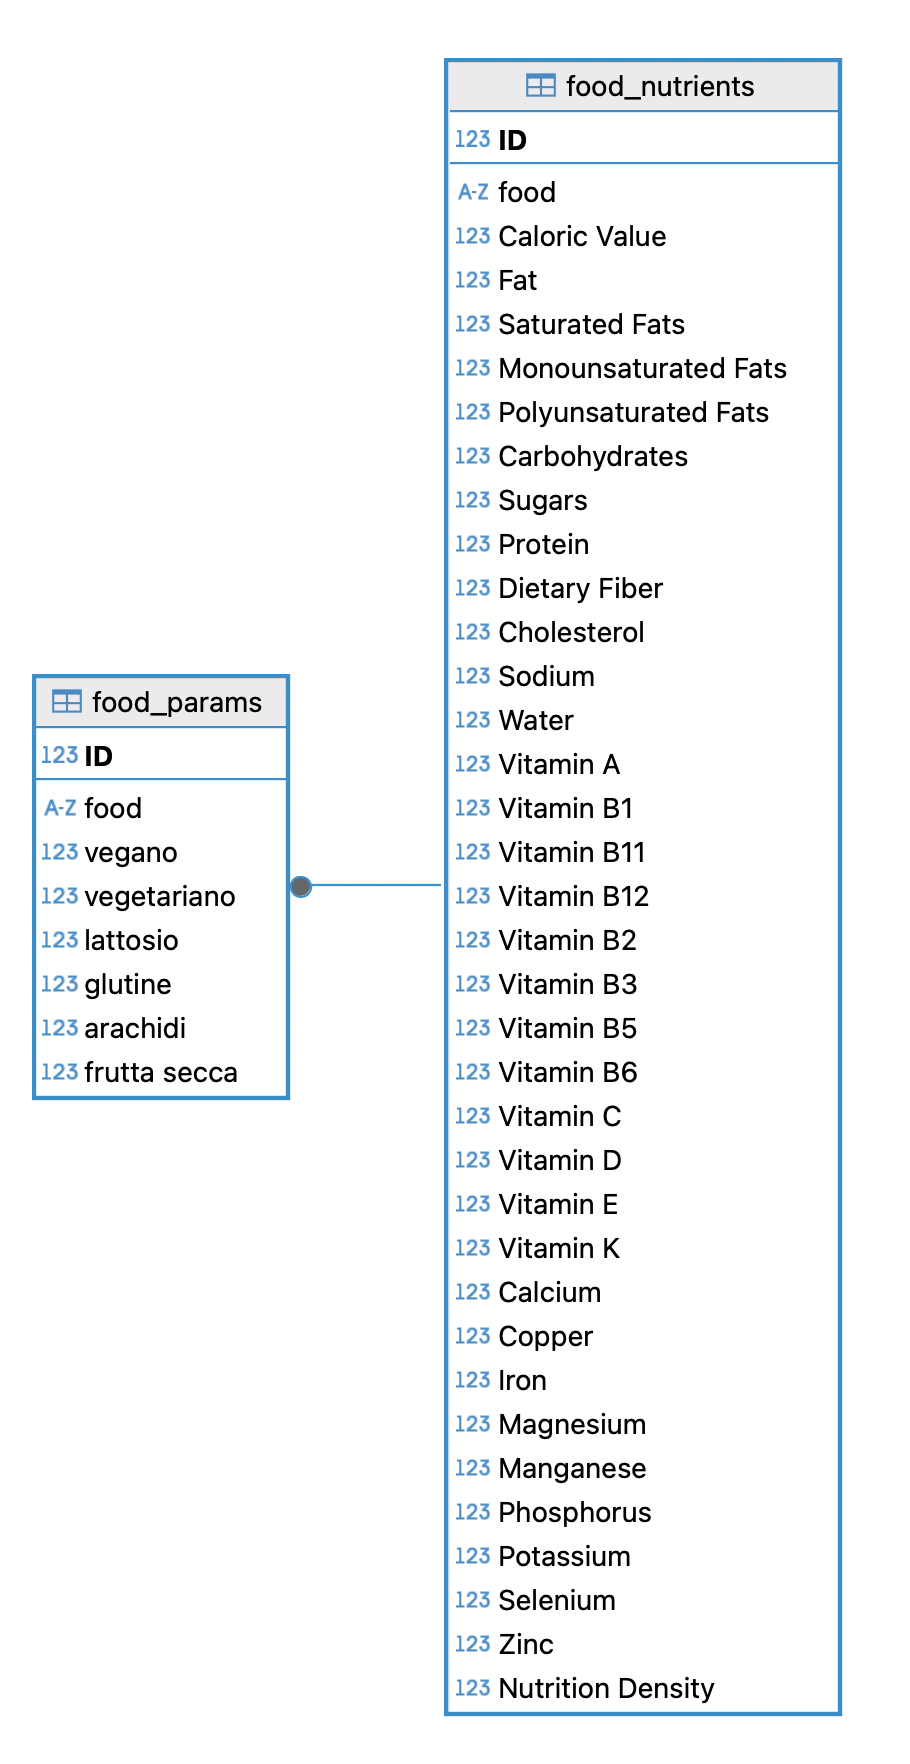
\includegraphics[width=0.4\textwidth]{ER_diagram.png}
    \caption{Diagramma ER del \textit{database}}
    \label{fig:er_diagram}
\end{figure}

\subsection{Criticità}
Inizialmente, si pensava che il \textit{dataset} potesse essere facilmente reperito; tuttavia, già in fase di ricerca è emerso che nessuno dei \textit{dataset} disponibili soddisfaceva integralmente tutti i requisiti necessari. In particolare, non esisteva un dataset dotato di informazioni complete, comprensive di dettagli sui nutrienti, valori di porzione tipica e categorizzazioni esplicative (ad es. etichette per prodotti vegani, latticini, ecc.). Di conseguenza è stato necessario selezionare un \textit{dataset} accettabile e adattarlo mediante processi di \textit{data cleaning} e \textit{data management}. Tale esigenza di intervento rappresenta una criticità rilevante: se in futuro si volesse implementare questo \textit{tool} in un contesto commerciale, sarebbe indispensabile sviluppare un \textit{dataset ad hoc}, utilizzando risorse e mezzi significativi per garantire la completezza, l’accuratezza e l’affidabilità dei dati.


% (Sottocapitoli da definire in seguito)

% ====================================================
% CAPITOLO 4
% ====================================================
\section{Descrizione ad alto livello delle strutture dati e degli algoritmi utilizzati}

\subsection{Struttura del Progetto}
Il progetto è realizzato in Python e segue l'architettura \textbf{MVC (Model-View-Controller)}, che consente di organizzare il codice suddividendo le responsabilità in moduli specifici, facilitando la manutenzione e l'estensione delle funzionalità.

\begin{figure}[h!]
    \centering
    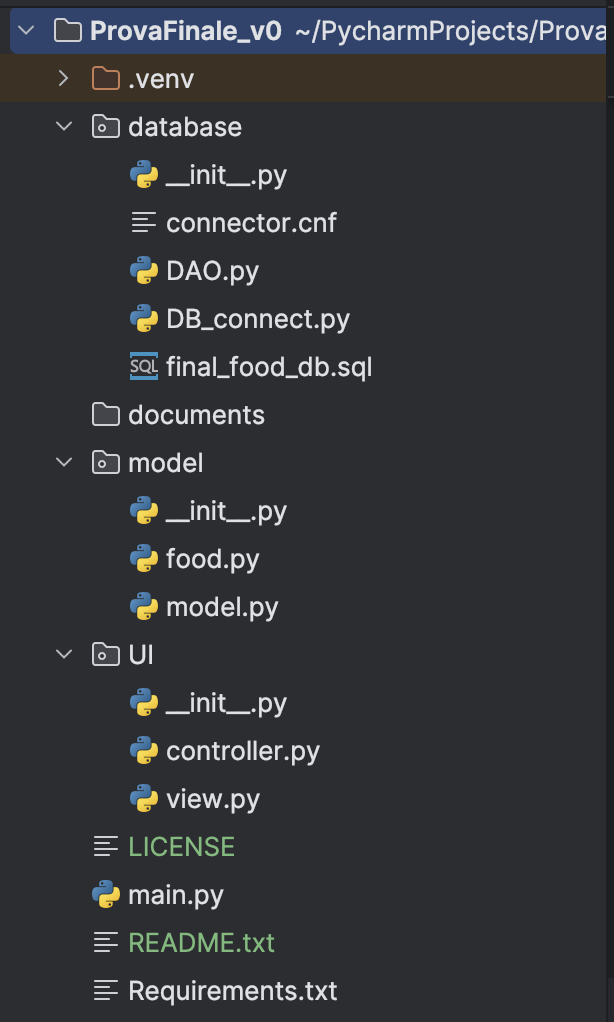
\includegraphics[width=0.2\textwidth]{file_tree.png}
    \caption{Struttura delle cartelle del progetto}
    \label{fig:file_tree}
\end{figure}


\textbf{Package Model: Gestione dei Dati e Logica di Business} \\
\begin{itemize}
    \item \textbf{model.py:} implementa le funzioni per il calcolo del Basal Metabolic Rate (BMR) mediante la formula di Mifflin-St Jeor e per il calcolo del Total Daily Energy Expenditure (TDEE) in base al livello di attività. Inoltre, fornisce metodi per il recupero e il filtraggio dei dati alimentari e per il calcolo dei fabbisogni nutrizionali, definendo un benchmark personalizzato.
    \item \textbf{food.py:} definisce la classe \texttt{Food}, che incapsula le informazioni relative ad un prodotto alimentare (ID, nome, e valori nutrizionali quali calorie, grassi, proteine, carboidrati, fibre, micronutrienti, ecc.), utilizzando il tipo \texttt{decimal.Decimal} per garantire la precisione.
\end{itemize}

\textbf{Package UI: Interfaccia Utente e Controllo} \\
\begin{itemize}
    \item \textbf{view.py:}

Il file \texttt{view.py} rappresenta la componente di presentazione dell'applicazione ed è implementato estendendo la classe \texttt{ft.UserControl} della libreria Flet. La struttura del file è stata progettata in modo modulare per facilitare la manutenzione e l'estensione dell'interfaccia.

Nel costruttore (\texttt{\_\_init\_\_}), vengono inizializzate le variabili d'istanza che rappresentano i vari elementi grafici, quali i campi di input, i pulsanti, i grafici e le sezioni di personalizzazione. Vengono inoltre definiti alcuni parametri della pagina (dimensioni, tema, allineamento, possibilità di ridimensionamento e scroll) per garantire una configurazione ottimale dell'interfaccia.

La costruzione dell'interfaccia è suddivisa in metodi privati (es.
\texttt{\_build\_row\_activity()}), ognuno dei quali si occupa di creare una specifica sezione della pagina. Questa organizzazione modulare rende il codice più leggibile e consente di isolare facilmente le modifiche a specifiche aree dell'interfaccia senza impattare sull'intera struttura.

Infine, il metodo \texttt{load\_interface()} funge da punto di ingresso per l'assemblaggio complessivo dell'interfaccia, richiamando in sequenza i metodi privati per costruire e aggiungere i componenti alla pagina. L'utilizzo di \texttt{Container} con padding, spaziatura e border radius uniformi garantisce un layout coerente e visivamente gradevole. La struttura del file \texttt{view.py} è studiata per separare nettamente la definizione degli elementi UI dalla logica di aggiornamento della pagina, assicurando così una facile integrazione con il controller e il modello.

    \item \textbf{controller.py:} implementa la logica di controllo, mediando tra il \texttt{Model} e la \texttt{View}. Il controller gestisce la validazione degli input, il calcolo del fabbisogno energetico, l'attivazione dell'algoritmo di ottimizzazione e la personalizzazione della lista della spesa.
\end{itemize}

\textbf{Database: (file di gestione del \textit{database})} \\
La cartella \texttt{database} contiene:
\begin{itemize}
    \item \texttt{DAO.py}: La classe \texttt{DAO} centralizza le operazioni di accesso al database, eseguendo query e trasformando i dati in oggetti \texttt{Food}. I metodi principali sono: 
        \begin{itemize}
        \item \texttt{getAllFood()} – restituisce l’elenco completo dei prodotti alimentari.
        \item \texttt{getFoodPers(switches\_state)} – estrae i dati filtrati in base alle preferenze dell’utente.
        \item \texttt{getFoodByNutrient(nutrient)} – restituisce una lista di alimenti ordinati in base a un particolare micronutriente.
        \end{itemize}
    \item \texttt{connector.cnf}: file di configurazione con le credenziali di accesso al database.
    \item \texttt{DB\_connect.py}: gestisce la connessione al database tramite un pool di connessioni.
    \item \texttt{DAO.py}: implementa la logica di accesso ai dati.
    \item \texttt{final\_food\_db.sql}: contiene lo schema e i dati di base.
\end{itemize}
Il file \texttt{main.py} rappresenta il punto di ingresso dell'applicazione, mentre \texttt{Requirements.txt} elenca le dipendenze (tra cui \textbf{Flet} e \textbf{PuLP}). I file \texttt{LICENSE} e \texttt{README.txt} forniscono le condizioni d'uso e le istruzioni per l'installazione.

\subsection{Algoritmi Coinvolti}

Il progetto utilizza formule matematiche per il calcolo del TDEE, del BMR e per la partizione dei nutrienti; tuttavia, l'algoritmo centrale è quello di ottimizzazione, implementato tramite un modello di Programmazione Lineare Intera Mista (MILP).

\subsubsection{Ottimizzazione}
L'approccio adottato consiste nel minimizzare la somma pesata delle deviazioni tra i valori nutrizionali ottenuti dalla combinazione degli alimenti e i target definiti, che si basano sul TDEE e sui dati biometrici dell'utente.
\begin{itemize}
    \item \textbf{Funzione Obiettivo:} \\
    La funzione obiettivo è definita come:
    \[
    \min \sum_{n \in N} w_n (d^+_n + d^-_n)
    \]
    dove \(w_n\) rappresenta il peso assegnato al nutriente \(n\) (ad esempio, 4 kcal/g per proteine e carboidrati, 9 kcal/g per i grassi, 0.5 per le fibre), e \(d^+_n\) e \(d^-_n\) sono le deviazioni positive e negative dal target.
    
    \item \textbf{Vincoli:} \\
    Per ogni nutriente \(n\), il modello impone:
    \[
    \sum_{i \in I} a_{in} x_i + d^-_n - d^+_n = T_n
    \]
    dove \(a_{in}\) è il contributo nutrizionale dell'alimento \(i\) per il nutriente \(n\), \(x_i\) è il numero di porzioni di alimento \(i\) e \(T_n\) è il target nutrizionale per \(n\). Inoltre, si impone che il numero totale di porzioni rientri in un intervallo prestabilito (ad es., da 5 a 15).

\end{itemize}

\subsubsection{Spiegazione Passo per Passo della Funzione \texttt{milp\_optimization}}

\begin{figure}[h!]
    \centering
    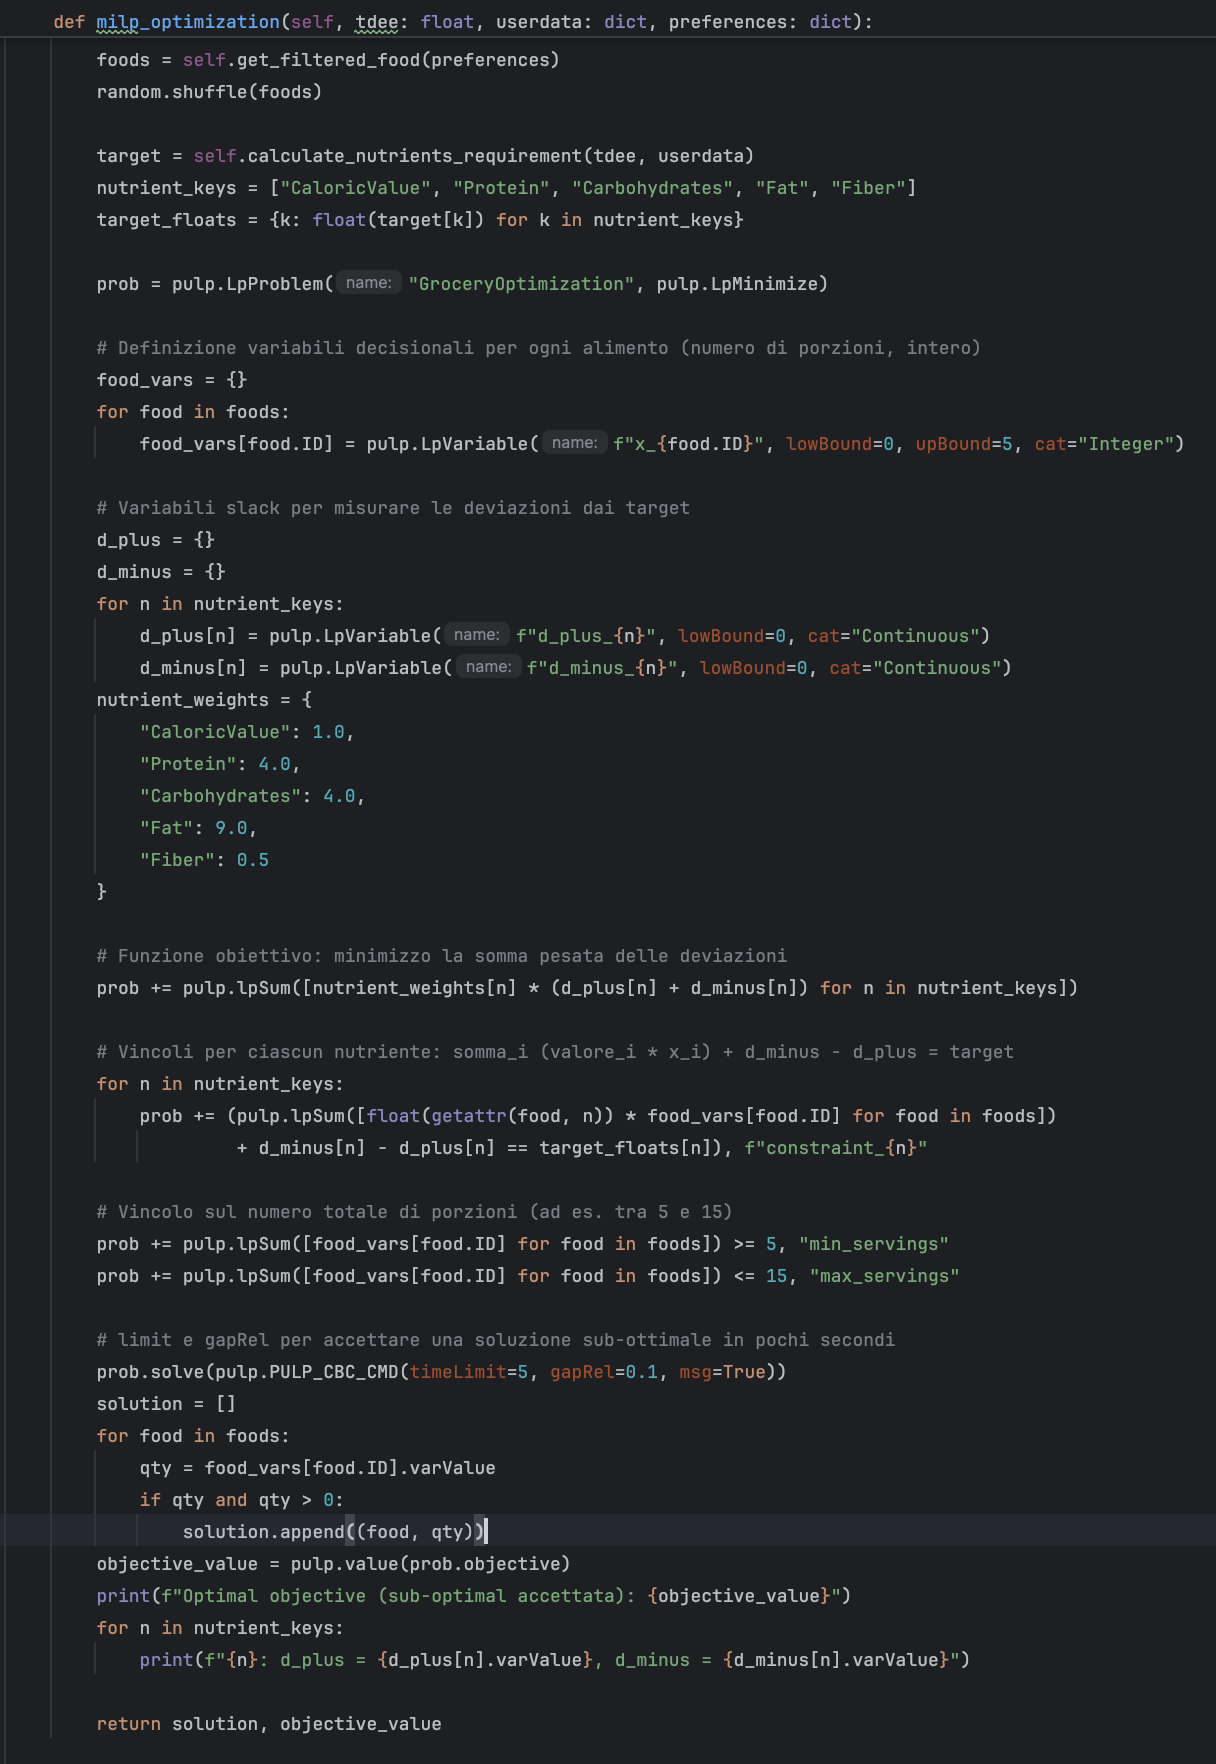
\includegraphics[width=0.7\textwidth]{milp_optimization.png}
    \caption{funzione milp optimization responsabile dell'ottimizzazione}
    \label{fig:milp_optimization}
\end{figure}

La funzione \texttt{milp\_optimization} si articola nei seguenti passaggi:
\begin{enumerate}
    \item \textbf{Acquisizione e Filtraggio dei Dati:} \\
    Vengono estratti e filtrati i prodotti alimentari dal database in base alle preferenze dell'utente, ottenendo una lista di oggetti \texttt{Food} che viene randomizzata per garantire soluzioni variegate.
    
    \item \textbf{Calcolo dei Target Nutrizionali:} \\
    Utilizzando il TDEE e i dati biometrici, il metodo \texttt{calculate\_nutrients\_requirement} definisce il benchmark nutrizionale personalizzato.
    
    \item \textbf{Definizione del Problema MILP:} \\
    Viene creato un oggetto \texttt{LpProblem} con l’obiettivo di minimizzare la somma pesata delle deviazioni, dove ciascuna deviazione è moltiplicata per il peso del nutriente corrispondente.
    
    \item \textbf{Definizione delle Variabili:} \\
    Per ogni alimento, viene definita una variabile intera che rappresenta il numero di porzioni, e per ogni nutriente, variabili slack \(d^+_n\) e \(d^-_n\) per misurare le discrepanze rispetto al target.
    
    \item \textbf{Imposizione dei Vincoli Nutrizionali:} \\
    Per ogni nutriente, la somma dei contributi degli alimenti selezionati, corretta dalle variabili slack, deve essere uguale al target nutrizionale.
    
    \item \textbf{Vincoli sul Totale delle Porzioni:} \\
    Il modello impone che il numero totale di porzioni sia compreso in un intervallo realistico (ad esempio, da 5 a 15).
    
    \item \textbf{Risoluzione del Problema:} \\
    Il modello viene risolto utilizzando il solver CBC di PuLP, con un limite di tempo e un gap relativo per ottenere una soluzione sub-ottimale in tempi brevi.
    
    \item \textbf{Estrazione della Soluzione:} \\
    I valori delle variabili decisionali vengono raccolti per formare la lista della spesa ottimizzata, che viene restituita insieme al valore dell’obiettivo e alle deviazioni per ciascun nutriente.
\end{enumerate}




Questo approccio consente di individuare in maniera efficiente una combinazione di alimenti che si avvicini al target nutrizionale desiderato, minimizzando le discrepanze e garantendo un output valido per la generazione della lista della spesa.



% ====================================================
% CAPITOLO 5
% ====================================================

% ====================================================
% CAPITOLO 5
% ====================================================

\section{Esempi di Utilizzo e Video Dimostrativo}

\subsection{Videate in fase di utilizzo}

\subsubsection{Input utente (Screenshot 1)}
L’utente inserisce i propri dati biometrici (peso, altezza, età, genere) e il livello di attività fisica. Queste informazioni saranno utilizzate per calcolare il TDEE.

\begin{figure}[h!]
    \centering
    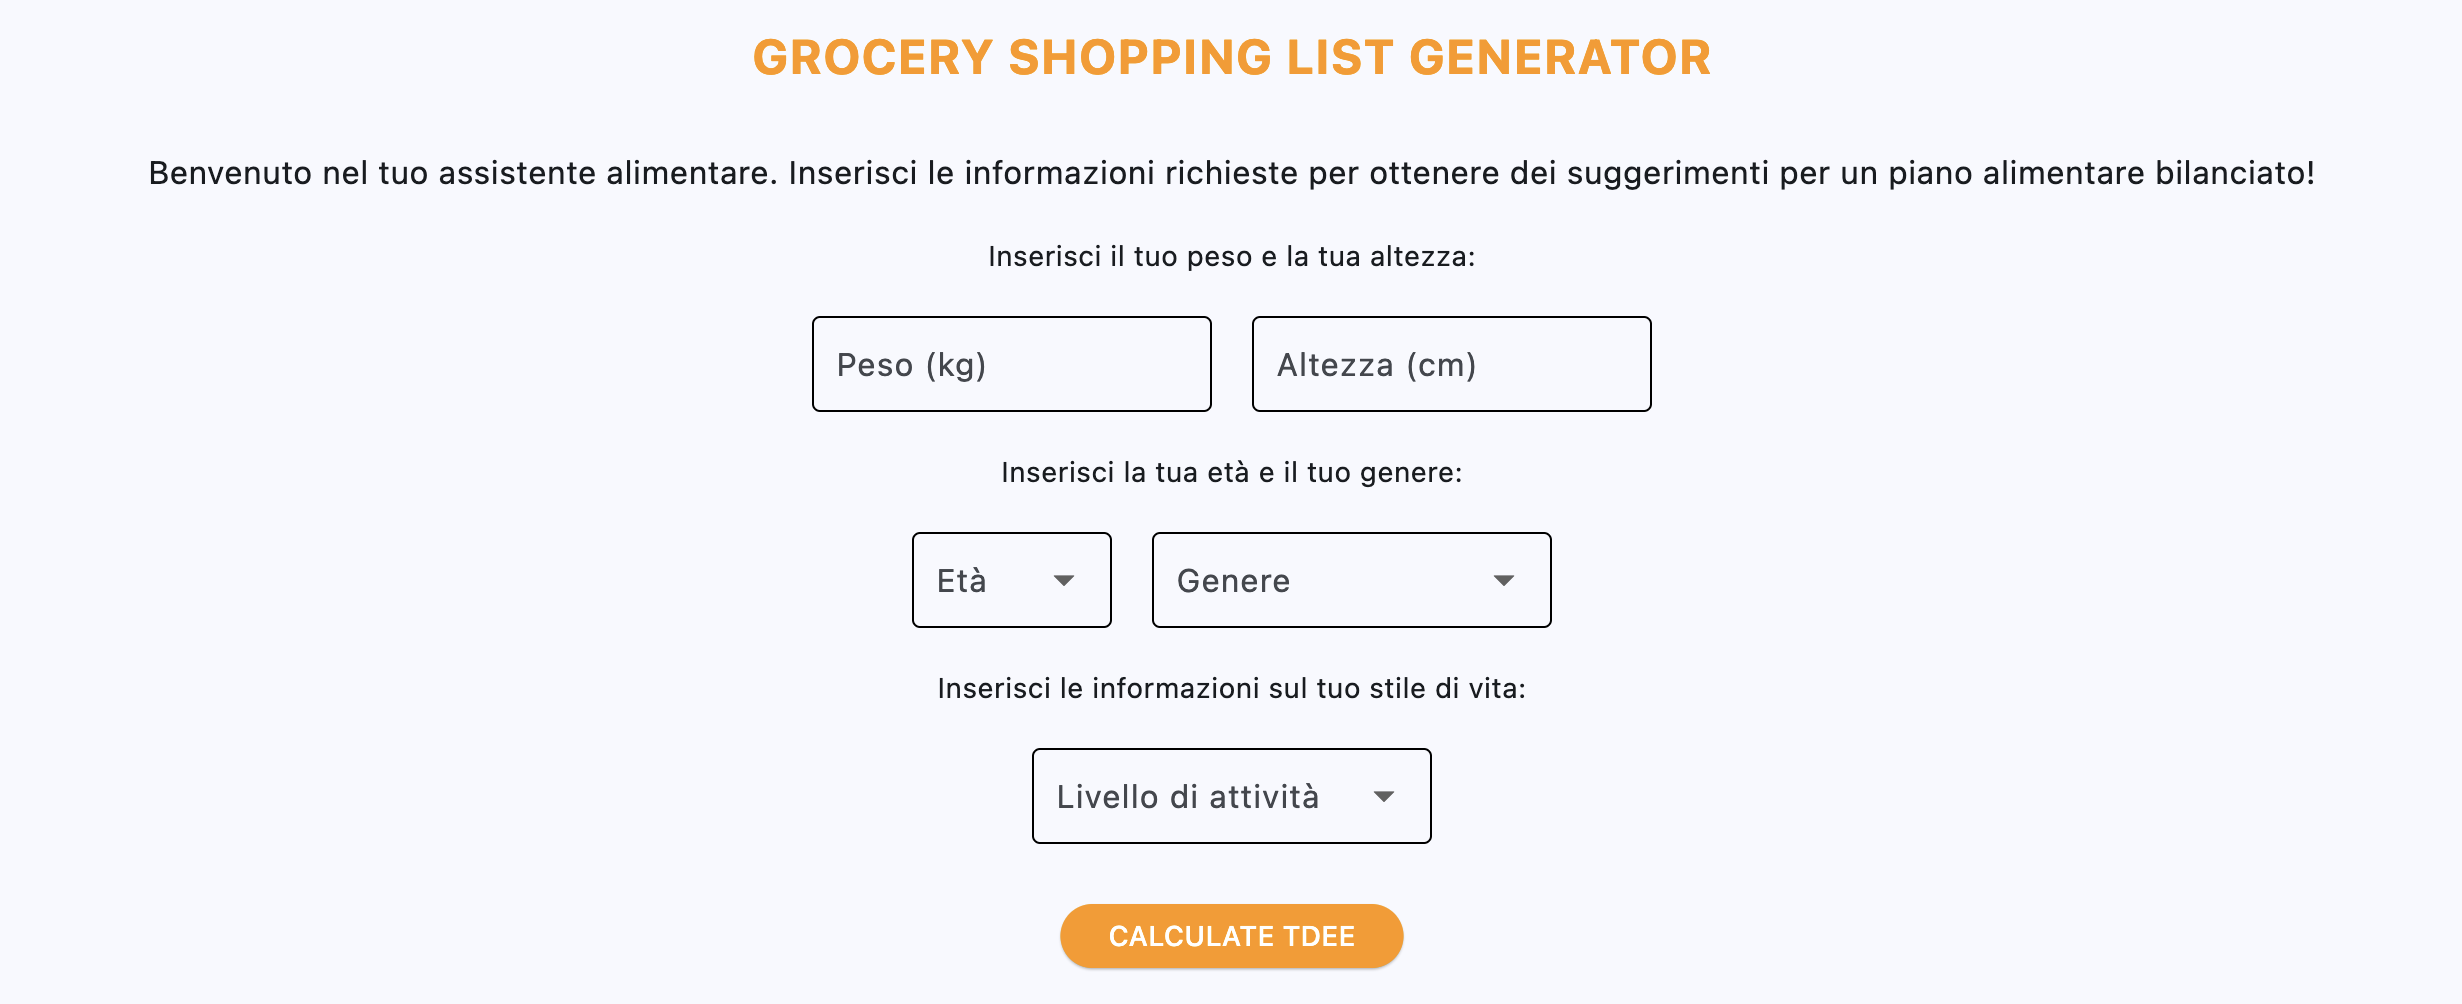
\includegraphics[width=0.8\textwidth]{input_utente.png}
    \caption{Schermata di Input Utente: Inserimento dei dati biometrici (peso, altezza, età, genere).}
    \label{fig:input_utente}
\end{figure}

\subsubsection{Calcolo TDEE (Screenshot 2)}
Una volta inseriti i dati, il sistema mostra il TDEE (fabbisogno calorico giornaliero), che potrà essere incrementato o decrementato di 100 kcal per adattarsi a esigenze specifiche.

\begin{figure}[h!]
    \centering
    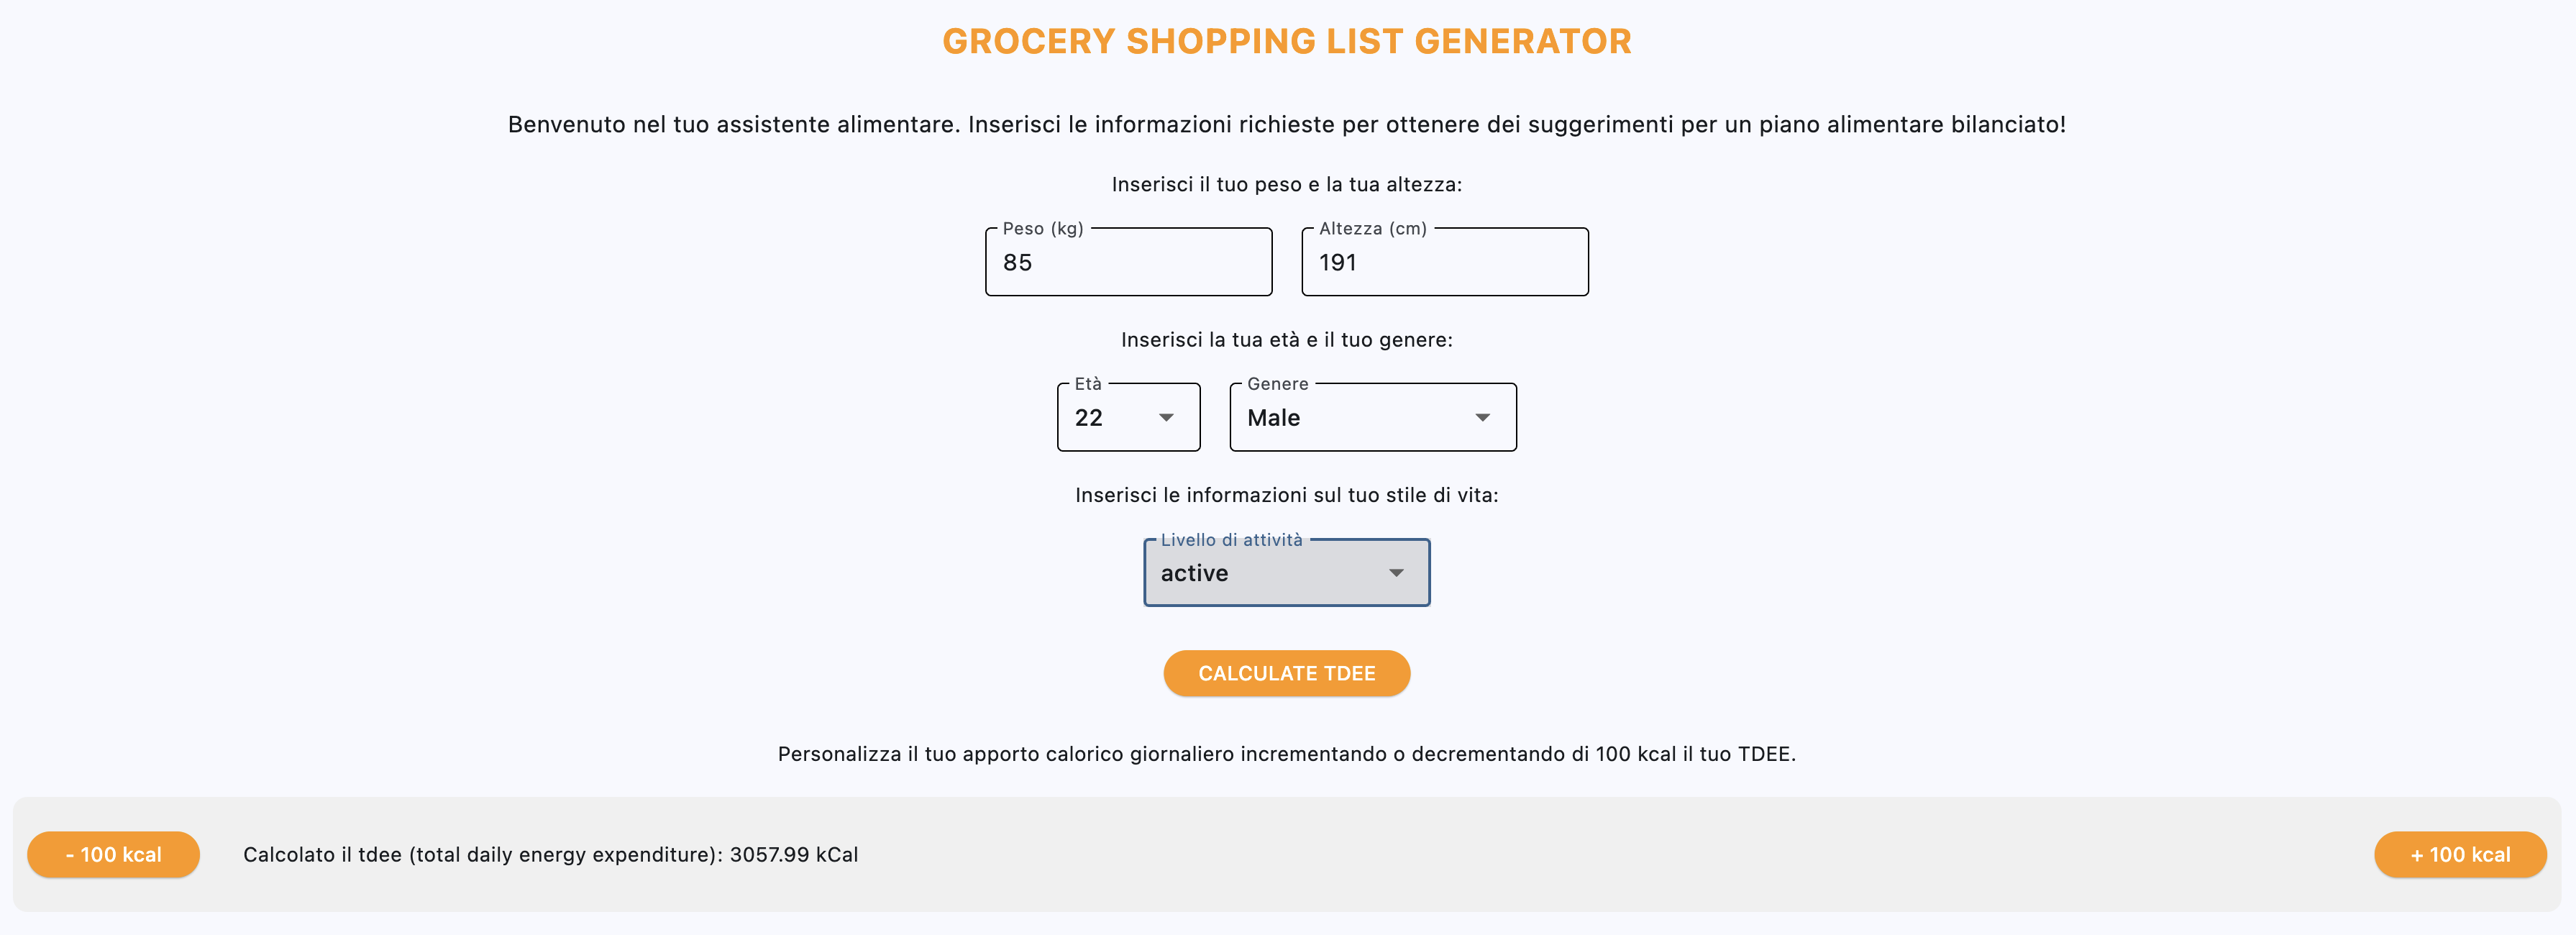
\includegraphics[width=0.8\textwidth]{calcolo_tdee.png}
    \caption{Schermata di Calcolo TDEE: Visualizzazione del fabbisogno calorico giornaliero calcolato.}
    \label{fig:calcolo_tdee}
\end{figure}

\subsubsection{Filtro alimenti (Screenshot 3)}
L’utente può attivare o disattivare vari switch per escludere categorie di cibi in base a preferenze dietetiche, intolleranze o allergie (ad es. lattosio, glutine, frutta secca).

\begin{figure}[h!]
    \centering
    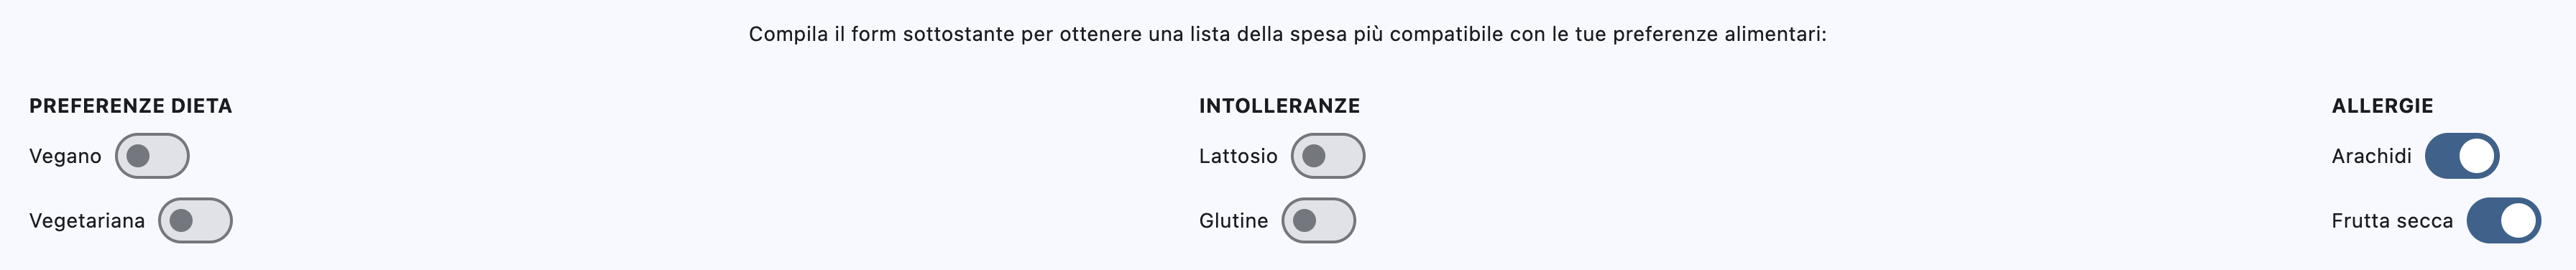
\includegraphics[width=0.8\textwidth]{filtro_alimenti.png}
    \caption{Schermata di Filtraggio Alimenti: Selezione delle preferenze alimentari tramite toggle.}
    \label{fig:filtro_alimenti}
\end{figure}

\subsubsection{Generazione output (Screenshot 4)}
Il sistema produce una lista della spesa ottimizzata, evidenziando per ogni alimento le porzioni suggerite, i nutrienti e l’apporto calorico.

\begin{figure}[h!]
    \centering
    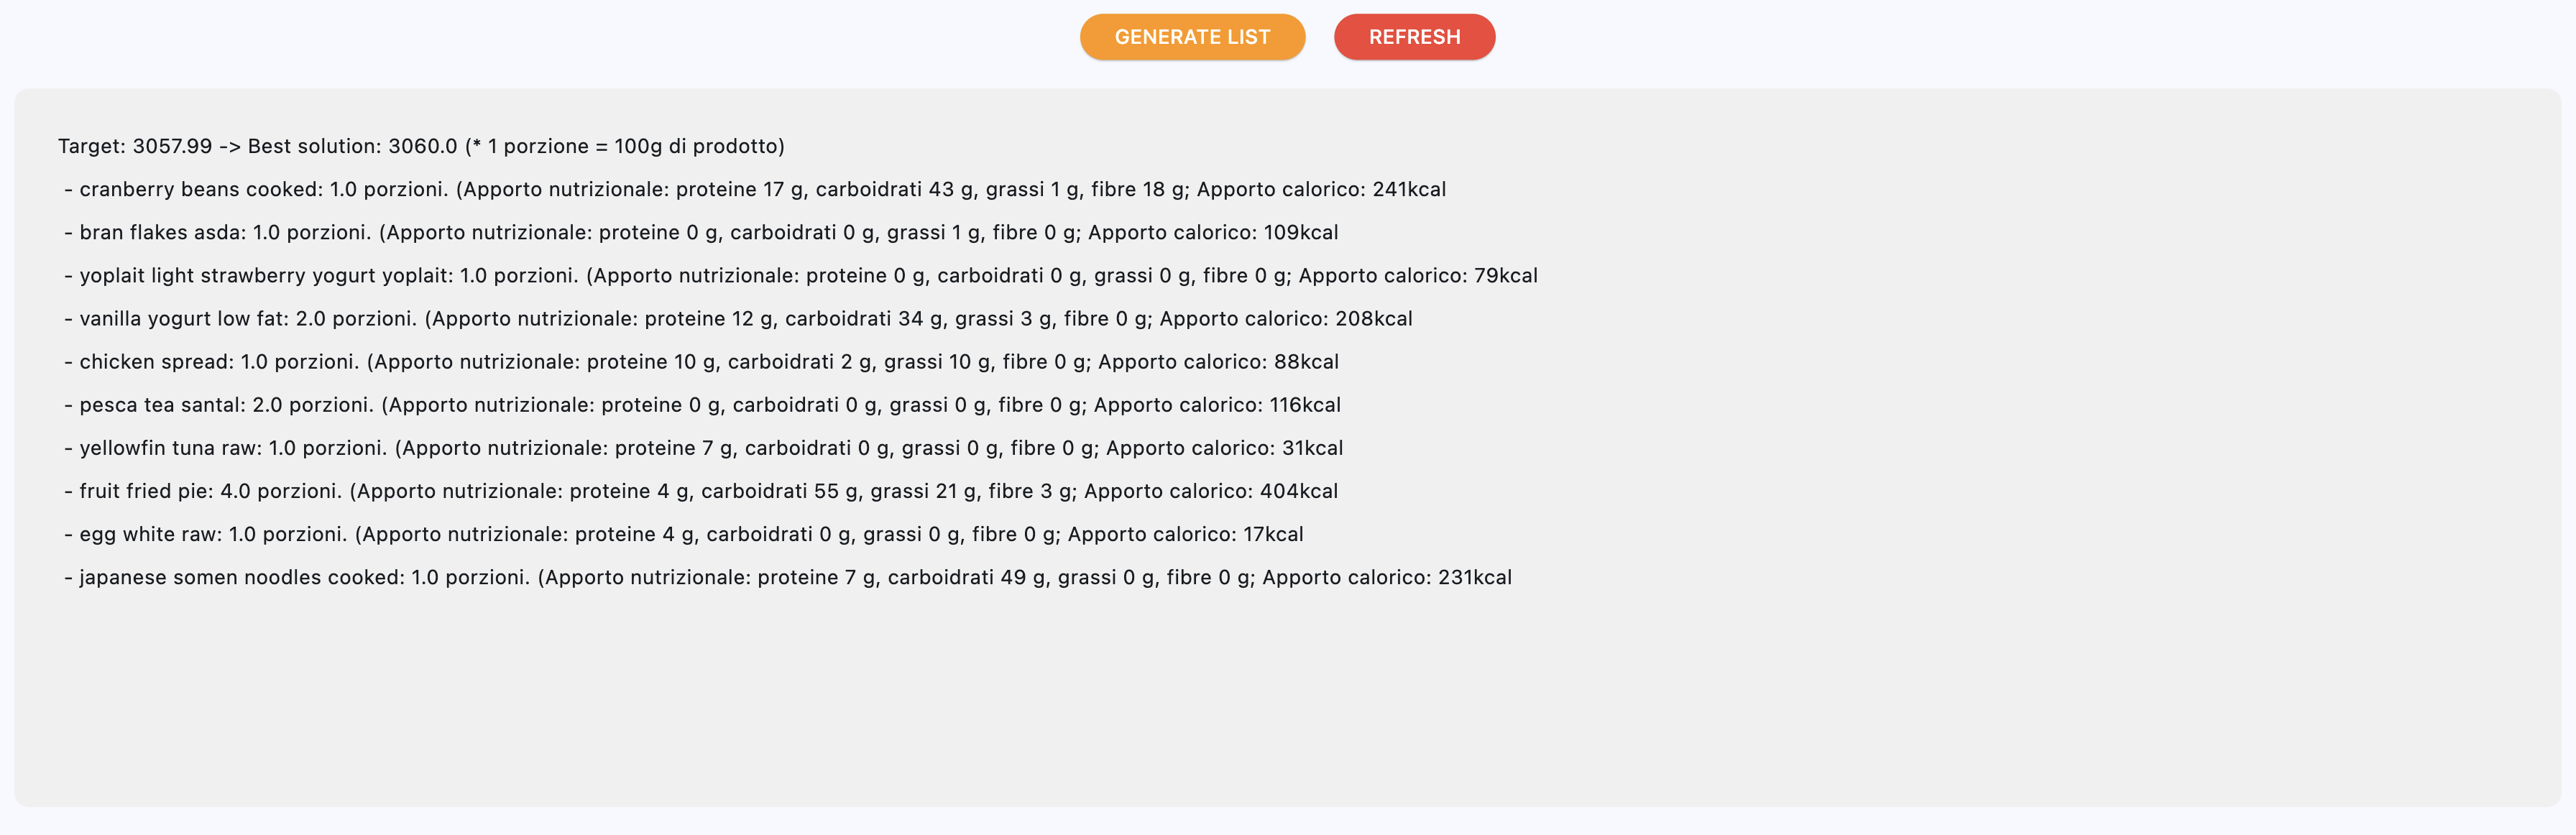
\includegraphics[width=1\textwidth]{generazione_output.png}
    \caption{Schermata di Generazione Output: Lista della spesa ottimizzata basata sul TDEE e sui dati inseriti.}
    \label{fig:generazione_output}
\end{figure}

\subsubsection{Personalizzazione output (Screenshot 5)}
L’utente può modificare la lista sostituendo alimenti indesiderati con prodotti nutrizionalmente simili, incrementando o decrementando il numero di porzioni, pur mantenendo l’equilibrio nutrizionale complessivo.

\begin{figure}[h!]
    \centering
    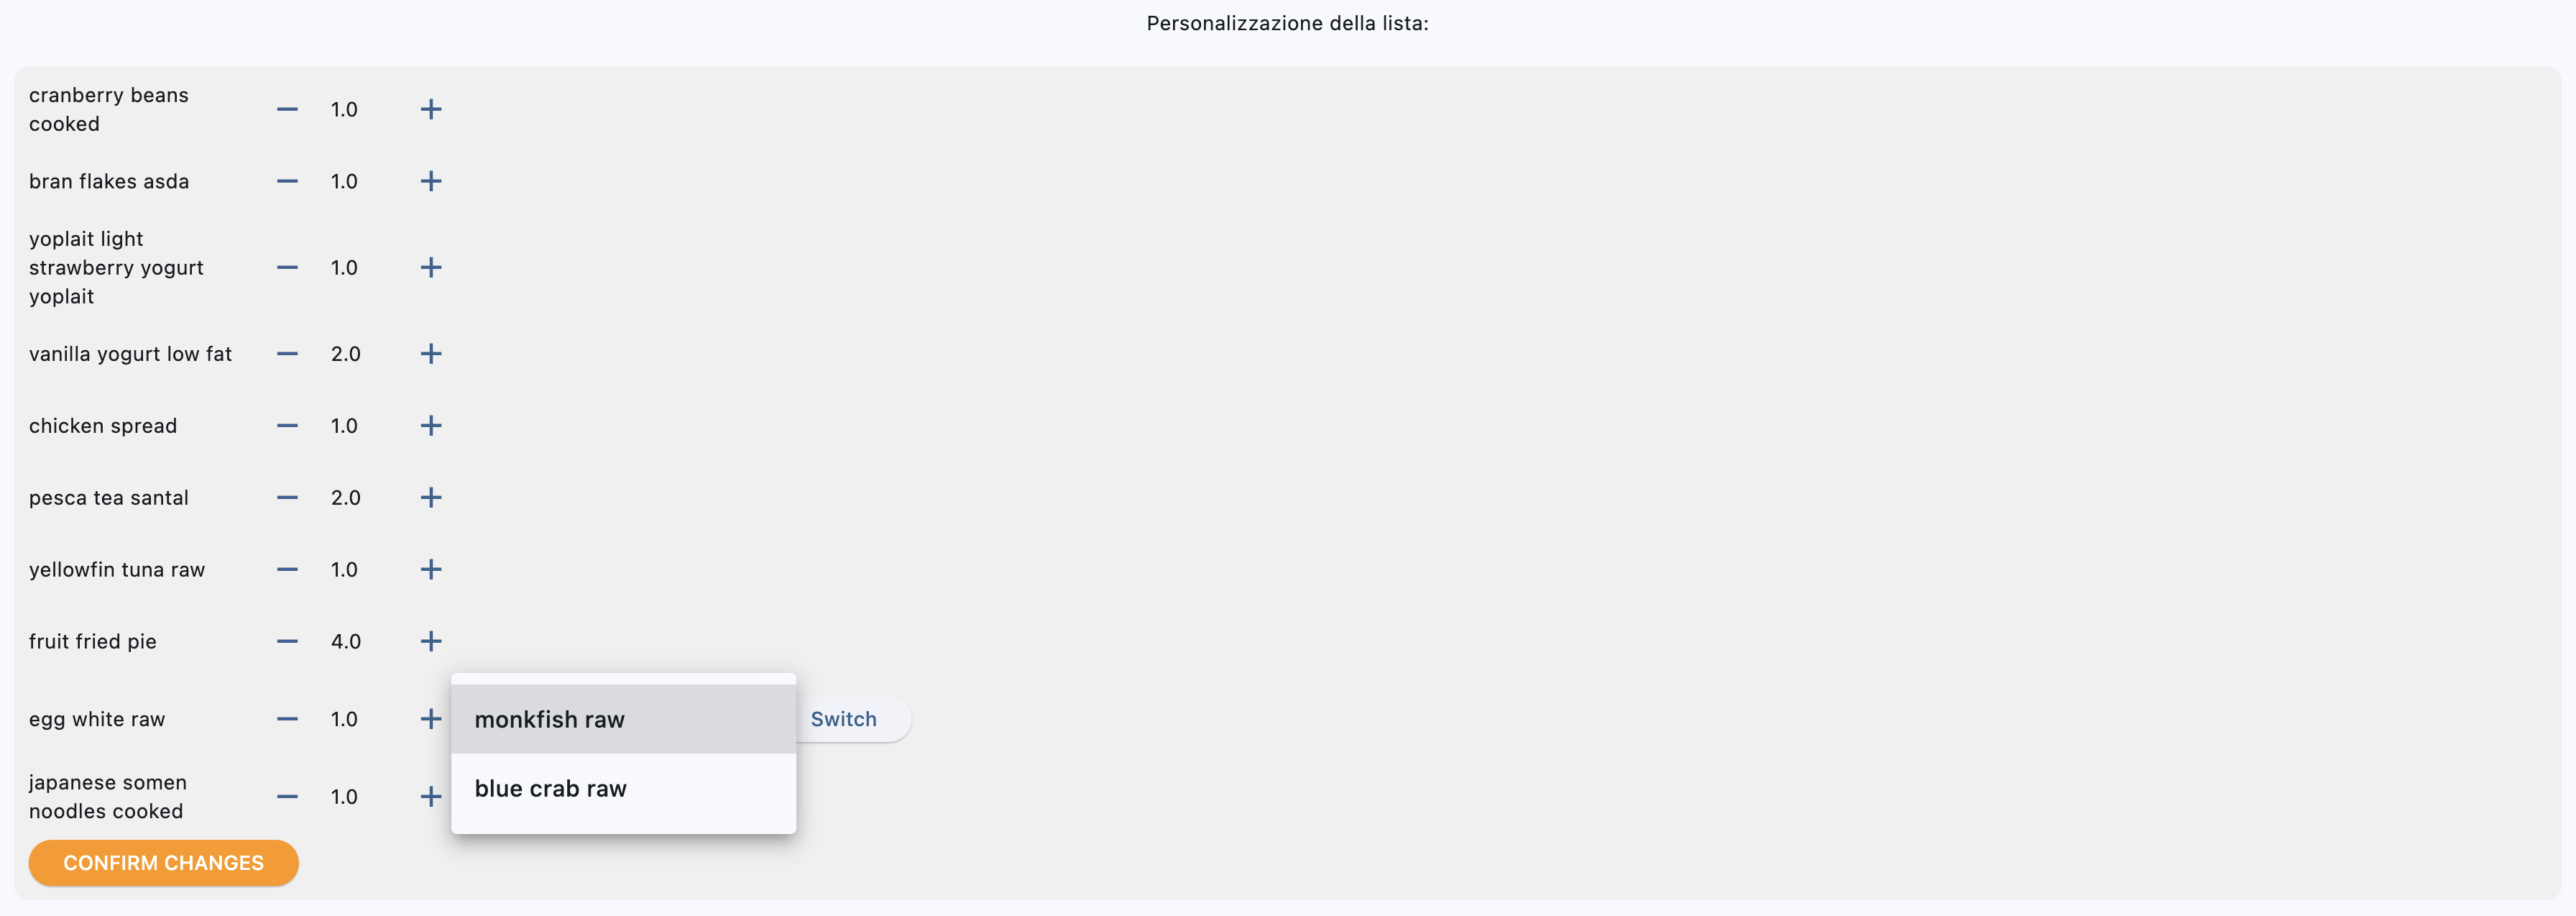
\includegraphics[width=1\textwidth]{personalizzazione_output.png}
    \caption{Schermata di Personalizzazione Output: Interfaccia per modificare la lista della spesa e sostituire alimenti.}
    \label{fig:personalizzazione_output}
\end{figure}

\subsubsection{Sezione micronutrienti (Screenshot 6)}
L’utente seleziona un micronutriente dal menu a tendina per visualizzare una breve descrizione informativa e un elenco di alimenti che lo contengono, ordinati in base al quantitativo presente.

\begin{figure}[h!]
    \centering
    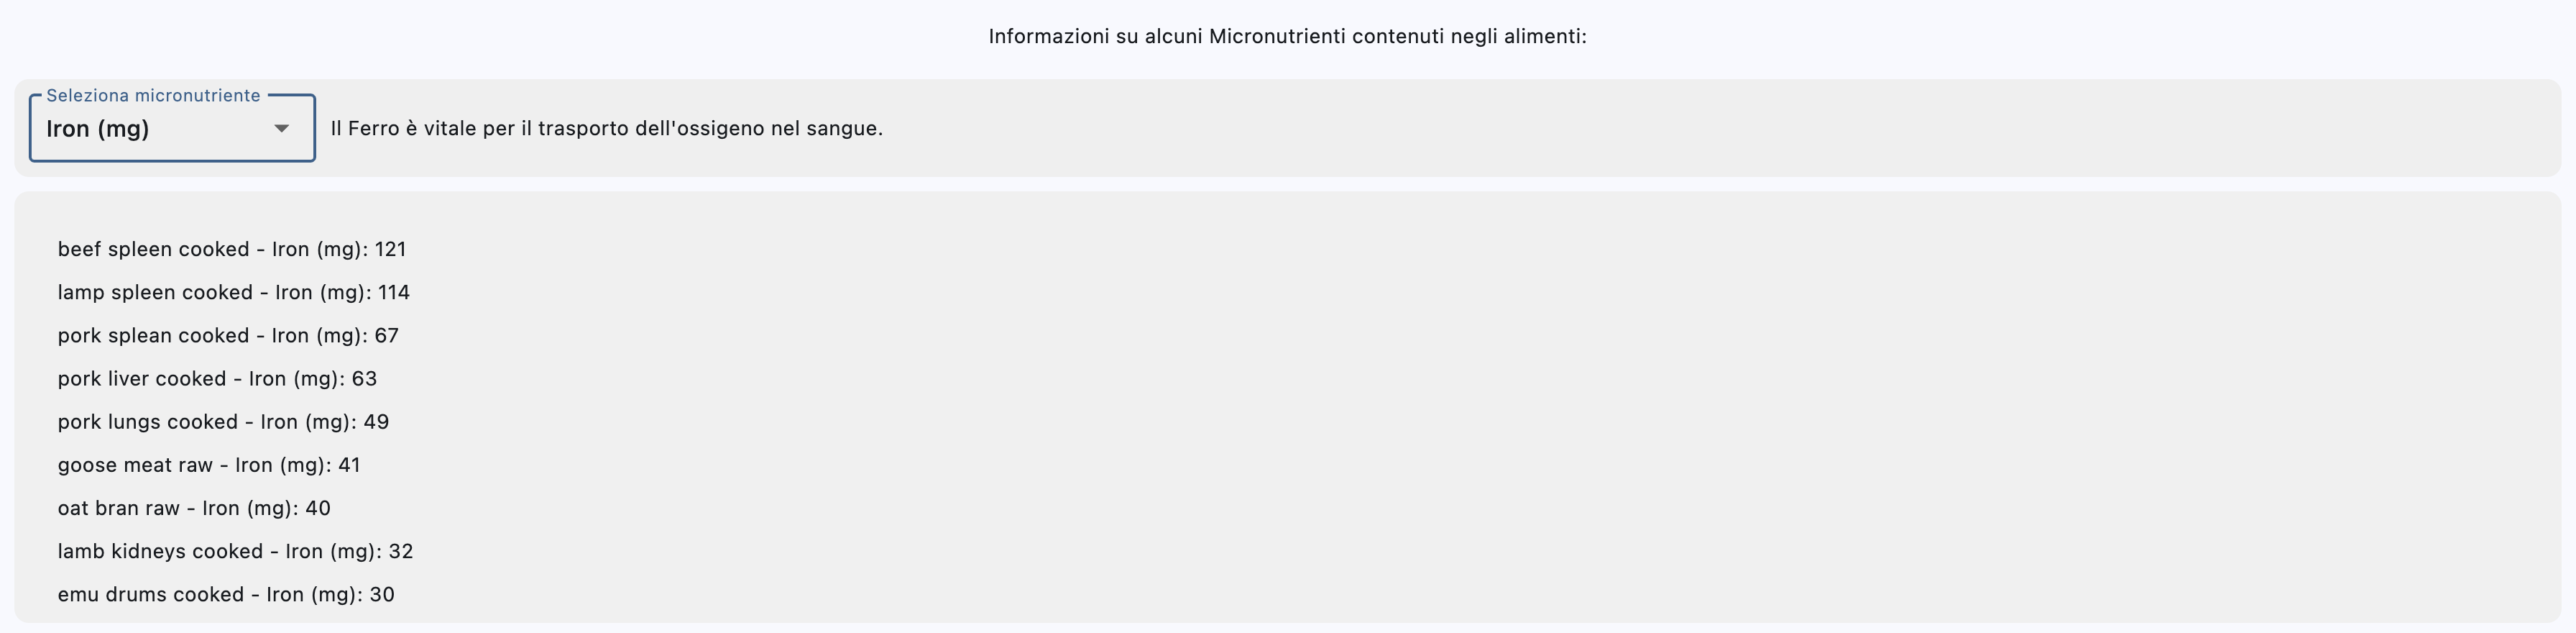
\includegraphics[width=1\textwidth]{sezione_micronutrienti.png}
    \caption{Schermata della Sezione Micronutrienti: Visualizzazione dei micronutrienti, relativo testo informativo e listview dei cibi.}
    \label{fig:sezione_micronutrienti}
\end{figure}

\subsection{Link al video dimostrativo}
Per una dimostrazione completa del funzionamento dell’applicazione, è disponibile il seguente video su YouTube:
\begin{center}
\url{https://youtu.be/zghf-64VrO0}
\end{center}



% (Sottocapitoli da definire in seguito)

% ====================================================
% CAPITOLO 6
% ====================================================

\section{Valutazione dei risultati ottenuti e conclusioni}

L’obiettivo principale di questo progetto è quello di semplificare la vita degli utenti automatizzando il processo di organizzazione e bilanciamento della dieta quotidiana. A partire dai dati biometrici e dalle preferenze alimentari, il sistema genera una lista della spesa ottimizzata che soddisfa un \textit{benchmark} nutrizionale personalizzato. Il flusso integrato comprende il calcolo del BMR e del TDEE, il filtraggio dei dati alimentari e l’applicazione di un algoritmo di ottimizzazione basato su un modello MILP, capace di minimizzare le discrepanze tra i valori nutrizionali ottenuti e quelli \textit{target}.

Durante lo sviluppo, sono emerse due criticità principali:
\begin{itemize}
    \item \textbf{Gestione del \textit{dataset}:} la mancanza di un \textit{dataset} completo ha richiesto intensi processi di \textit{data cleaning} e \textit{data management} per adattare i dati alle esigenze del progetto.
    \item \textbf{Complessità computazionale dell’ottimizzazione:} L’algoritmo MILP, sebbene efficace, richiede risorse computazionali significative, soprattutto con l’aumento del numero di variabili.
\end{itemize}

Il risultato finale dimostra che il sistema è in grado di generare soluzioni che si avvicinano ai \textit{target} nutrizionali in tempi ragionevoli, confermando la validità dell'approccio adottato. Questo strumento offre potenziali applicazioni sia in ambito individuale che commerciale, ad esempio come modulo integrabile in piattaforme di spesa \textit{online} atte a fornire consigli nutrizionali personalizzati.

\bigskip

In conclusione, il progetto ha raggiunto il suo obiettivo di automatizzare la pianificazione alimentare, semplificando un processo spesso trascurato e contribuendo al miglioramento della qualità della vita degli utenti. Le prospettive future includono il perfezionamento del \textit{dataset} e l’ottimizzazione dell'algoritmo per aumentare la scalabilità e la reattività, integrando ulteriori parametri nutrizionali e adattamenti dinamici basati sui \textit{feedback} degli utenti.


% (Sottocapitoli da definire in seguito)


% ====================================================
% CAPITOLO 7
% ====================================================

\section{LICENZA}

Questa relazione tecnica è distribuita con licenza \textbf{Creative Commons BY-NC-SA 4.0}.\\
Tu sei libero di:
\begin{itemize}
    \item \textbf{Condividere} -- riprodurre, distribuire, comunicare al pubblico, esporre in pubblico, rappresentare, eseguire e recitare questo materiale in qualsiasi mezzo e formato.
    \item \textbf{Modificare} -- remixare, trasformare il materiale e basarti su di esso per creare opere derivate.
\end{itemize}

Alle seguenti condizioni:
\begin{itemize}
    \item \textbf{Attribuzione:} Devi fornire una corretta attribuzione all’autore, riconoscendo la paternità dell’opera, includendo un link alla licenza e indicando se sono state apportate modifiche, in maniera ragionevole.
    \item \textbf{Non Commerciale:} Non puoi utilizzare il materiale per scopi commerciali.
    \item \textbf{Stessa Licenza:} Se remixi, trasformi o crei opere derivate, devi distribuire i tuoi contributi con la stessa licenza del materiale originale.
\end{itemize}

Per visualizzare una copia completa della licenza, visita: \url{https://creativecommons.org/licenses/by-nc-sa/4.0/}



\end{document}
